\chapter{Корреляционный анализ модовой структуры} \label{chapt3}
В ходе работы был предложен и проведён эксперимент по регистрации модовой структуры синхротронного излучения на European XFEL. Для эксперимента предлагалось взять ондуляторную линию SASE2 с одним закрытым ондулятором и с наилучшим разрешением монохроматора зарегистрировать распределение излучения в дальней зоне. Ондуляторная линия работала в однопучковом режиме, это значит, что излучение регистрировалось по пролёту одного электронного пуча и предполагается, что регистрируемый сигнал -- одна статистическая реализация интенсивность распределения синхротронного ондуляторного излучения. Однако, сколько продольных мод оставлял монохроматор и в конечном итоге усреднялось на детекторе, точно сказать не представляется возможным, потому что не известна информация о продольном распределении электронного пучка.

Практическая ценность такого эксперимента заключается в возможность реализовать неинвазивную диагностику электронного пучка вдоль всей ондуляторной линии SASE2. Поочерёдно закрывая каждый из 35 ондуляторов линии, измерив поперечное распределение интенсивности после монохроматора и рассчитав функцию взаимной когерентности, можно восстановить размеры электронного пучка в каждом ондуляторе.

\section{Моделирование}
В реальном эксперименте использовалась фундаментальная гармоника ондуляторного излучения с резонансом на $9.099$ эВ и кремниевым монохроматором на плоскости отражения $\textup{Si}(333)$. Источник излучения располагался на $206.8$ м от детектора. Оценить конфигурацию электронного пучка после ускорения в линейном ускорителе European XFEL не представлялось возможным\footnote{Пучки после линейного ускорителя обладают весьма не гауссовой формой,как это быват в накопительных кольцах.}, однако заявленный эмиттанс электронного пучка можно найти в \cite{schneidmiller_baseline_2018}, для моделирования был взят $1$ mm-mrad -- величина среднеквадратичного отклонения нормализованного эмиттанса, на энергии $14$ ГэВ, что отвечает размеру электронного пучка в источнике $30$ мкм при бета функции $26$. 

Смоделированное распределение интенсивности на расстоянии $206.8$ м от источника излучения выглядит следующим образом Рис.~\ref{fig:sim_single_shot}
\begin{figure}[H] 
	\centering 	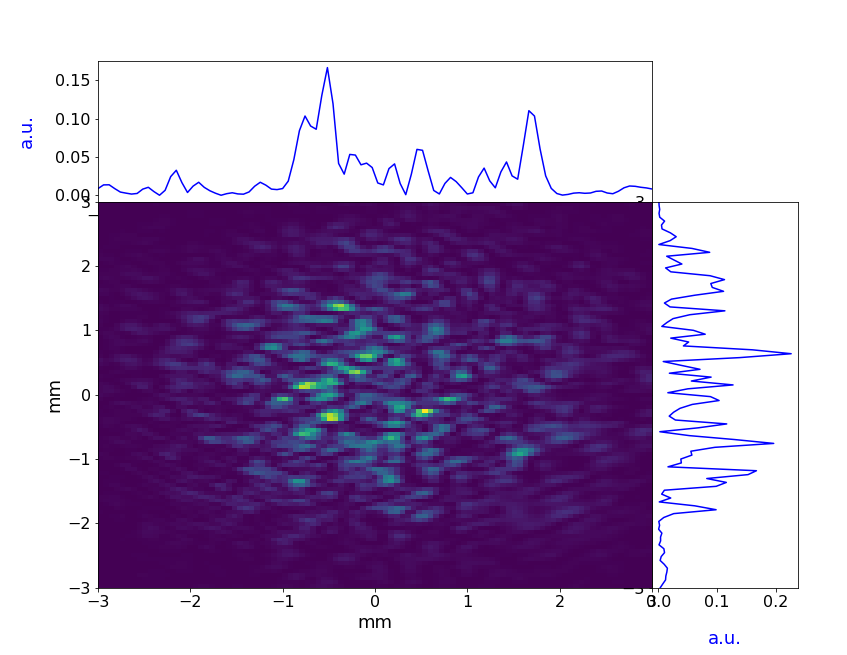
\includegraphics[width=0.99\linewidth]{sim_single_shot.png}
	\caption{Распределение интенсивности смоделированного сигнала от одного из ондуляторов SASE2 на расстоянии $206.8$ м от источника излучения}
	\label{fig:sim_single_shot}
\end{figure}

Для определения поперечной длины когерентности можно пользоваться функциями взаимной когерентности как первого~\ref{eq:g1}, так и второго порядка:
\begin{align}
	g^{(2)} (r_1, r_2, \omega) = \cfrac{\big \langle \bar{I}(r_1, \omega) \bar{I}(r_2, \omega) \big \rangle}{\big \langle \bar{I}(r_1, \omega)\big \rangle \big \langle\bar{I}(r_2, \omega) \big \rangle}, 
	\label{eq:g2} 
\end{align}
где $\bar{I}(r) = \bar{E}(r)\bar{E}^*(r)$. Здесь стоит отметить, что для определения длины когерентности измеренного сигнала использовалась функция второго порядка, так как детектором регистрировалось именно интенсивность излучения, а не сама напряжённость электромагнитного поля.

Функция взаимной когерентность первого порядка представлена на Рис.~\ref{fig:sim_g1} 
\begin{figure}[H] 
	\centering 	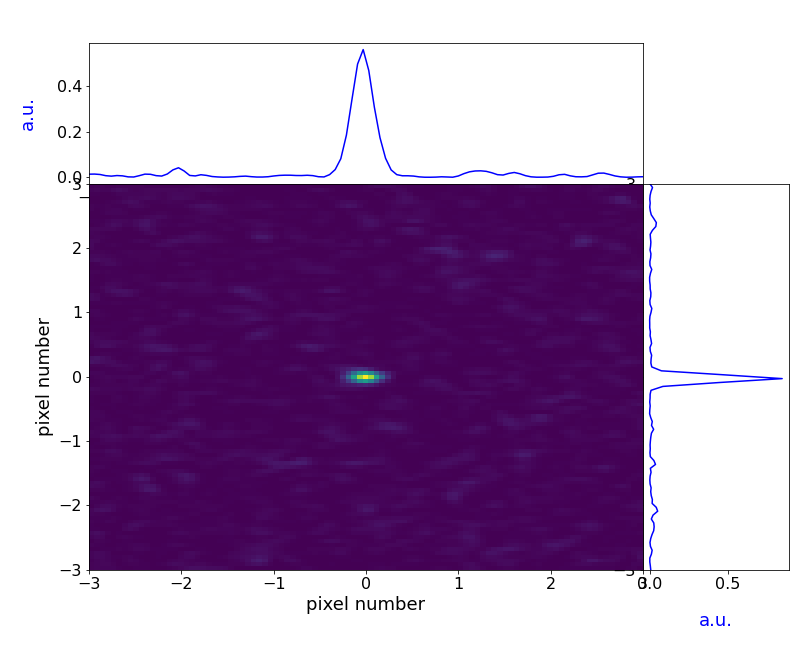
\includegraphics[width=0.99\linewidth]{sim_g1.png}
	\caption{Распределение функции взаимной когерентности первого порядка от сигнала на Рис.~\ref{eq:g1}}
	\label{fig:sim_g1}
\end{figure}
Функция взаимной когерентности второго порядка представлена на Рис.~\ref{fig:sim_g2}
\begin{figure}[H] 
	\centering 	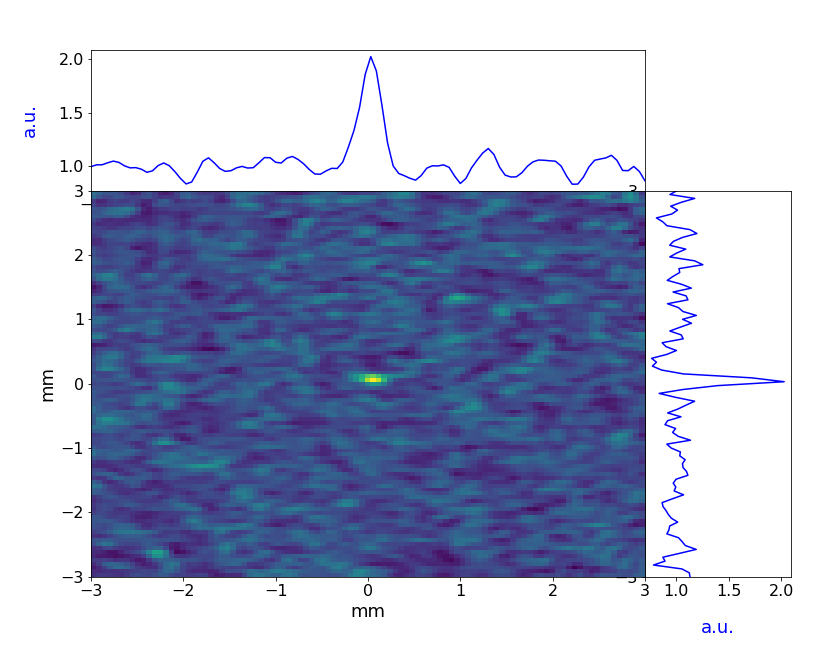
\includegraphics[width=0.99\linewidth]{sim_g2.png}
	\caption{Распределение функции взаимной когерентности первого порядка от сигнала на Рис.~\ref{eq:g2}}
	\label{fig:sim_g2}
\end{figure}
Именно такое распределение ожидается увидеть при детектировании сигнала в реальном эксперименте.
\section{Экспериментальные данные}
В эксперименте была набрана статистика из 424 реализаций поля, усреднённый сигнал представлен на Рис.~\ref{fig:exp_signal}. Особенности снятого сигнала заключаются в критически малом соотношении сигнал/шум, а так же в специфических "волнах" на детекторе \rr{добавить рисунок с одно реализацией, где видны эти волны}.
\begin{figure}[H] 
	\centering 	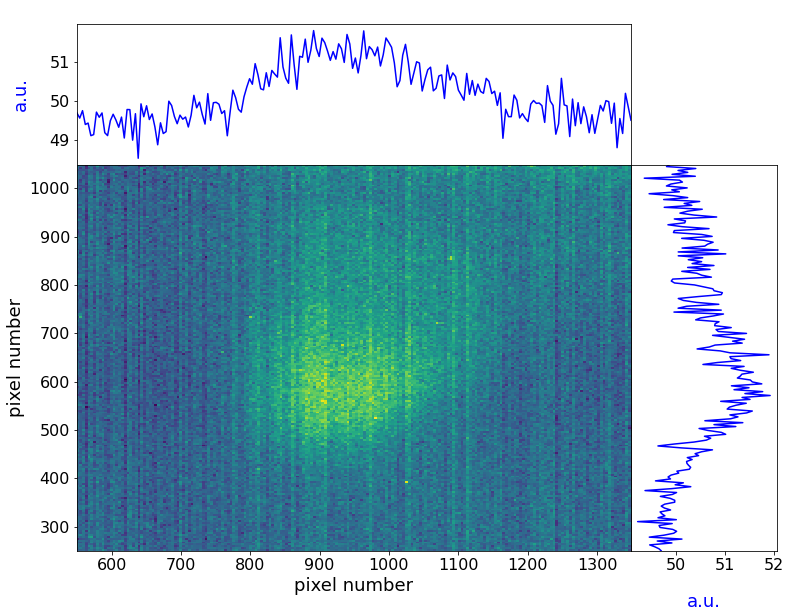
\includegraphics[width=0.99\linewidth]{exp_signal.png}
	\caption{\rr{Подпись}}
	\label{fig:exp_signal}
\end{figure}
После проведения корреляционного анализа \rr{...} 
\begin{figure}[H] 
	\centering 	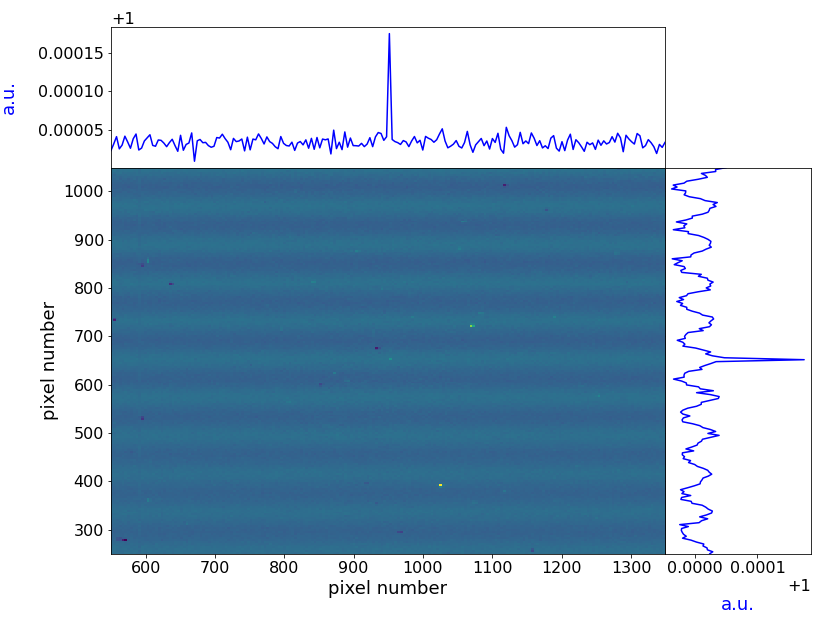
\includegraphics[width=0.99\linewidth]{exp_g2.png}
	\caption{\rr{Подпись}}
	\label{fig:exp_g2}
\end{figure}

\section{Анализ результатов}

\newpage
%============================================================================================================================

\clearpage